	\subsection{LP coefficients clustering}

		\subsubsection{K-Means}
			
			As K-Means allows for the number of clusters to be defined, and we know that there are 4 in the original dataset, K-Means is used to find 4 clusters.
			
			\begin{table}[h!]
				\centering
				\begin{tabular}{|c|c|c|}
					\hline
					& \textbf{Number of clusters} & \textbf{Number of initializations}\\
					\hline
					\textbf{Original LP coefficients} & 4 & 10\\
					\hline
					\textbf{PCA LP coefficients} & 4 & 10\\
					\hline
					\textbf{UMAP LP coefficients} & 4 & 10\\
					\hline
				\end{tabular}
				\caption{K-Means hyperparameter configuration for c coefficients clustering}
			\end{table}
		
			The results are the following:
			
			\begin{figure*}[ht!]
				\centering
				\subfloat[Original cluster densities]{%
					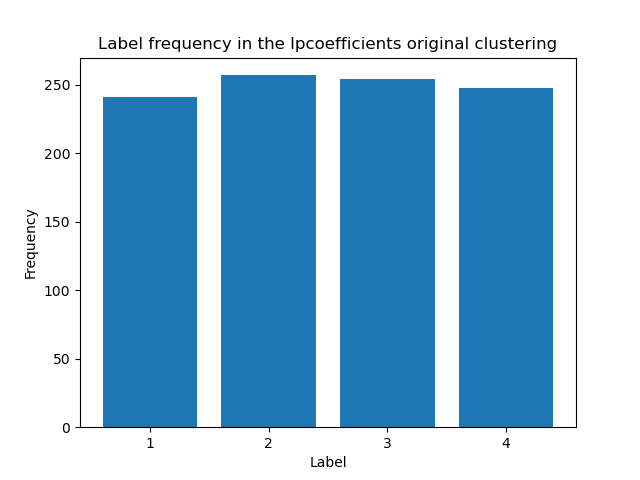
\includegraphics[width=0.45\textwidth]{mdid-lpcoefficientsoriginaldensity.png}}
				\hspace{\fill}
				\subfloat[K-Means clusters densities]{%
					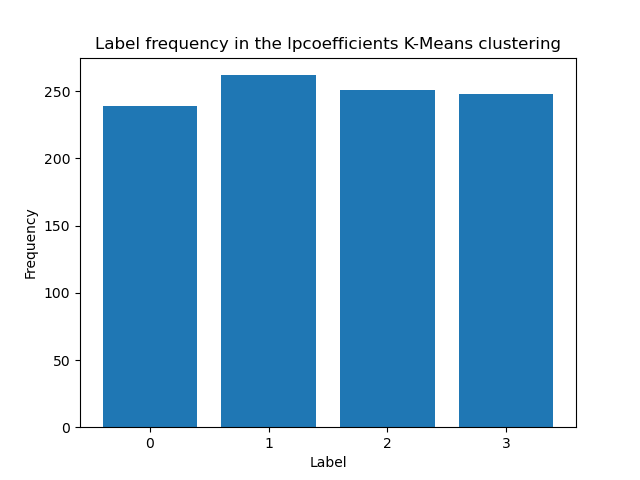
\includegraphics[width=0.45\textwidth]{mdid-lpcoefficientsK-Meansdensity.png}}\\
				\subfloat[Original clusters]{%
					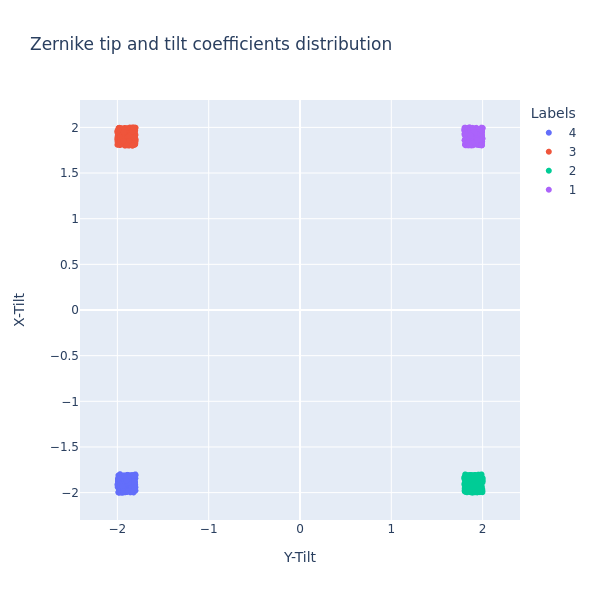
\includegraphics[width=0.45\textwidth]{mdid-originalclusters.png}}
				\hspace{\fill}
				\subfloat[K-Means clusters]{%
					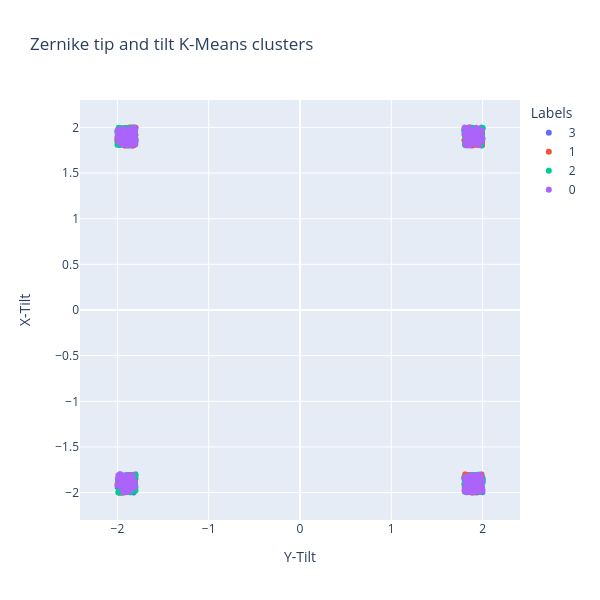
\includegraphics[width=0.45\textwidth]{mdid-lpcoefficientsK-Meansclusters.png}}\\
					
				\subfloat[Original cluster samples]{%
					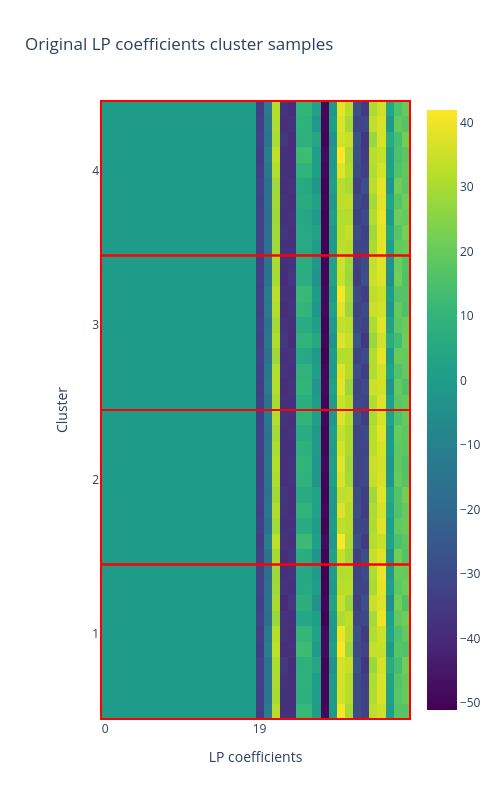
\includegraphics[width=0.4\textwidth]{mdid-lpcoefficientsoriginalgridclusters.png}}
				\hspace{\fill}
				\subfloat[K-Means cluster samples]{%
					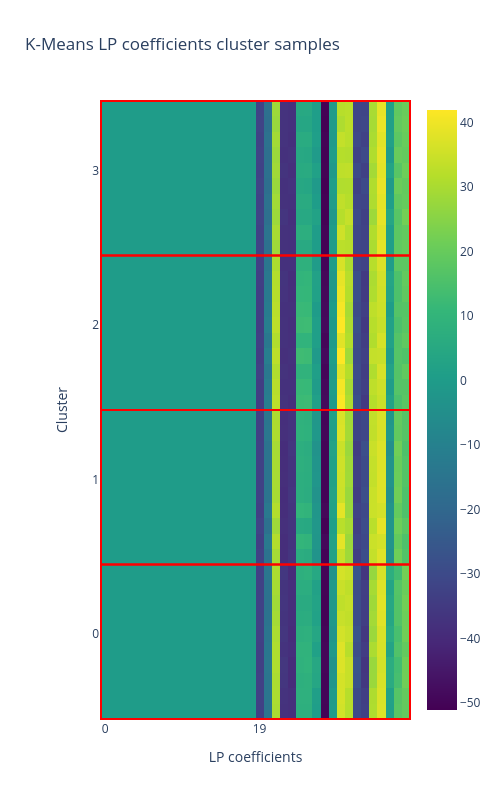
\includegraphics[width=0.4\textwidth]{mdid-lpcoefficientsK-Meansgridclusters.png}}
				\caption{Comparison between original clustering and K-Means clustering from original LP coefficients}
			\end{figure*}
			\FloatBarrier
		
			\begin{figure*}[ht!]
				\centering
				\subfloat[Original cluster densities from PCA]{%
					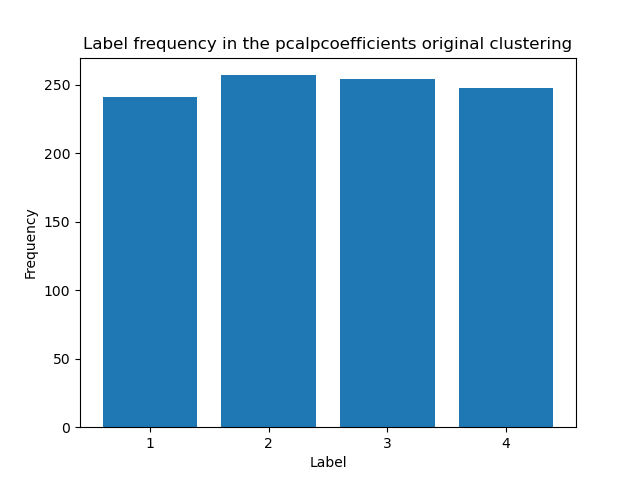
\includegraphics[width=0.45\textwidth]{mdid-pcalpcoefficientsoriginaldensity.png}}
				\hspace{\fill}
				\subfloat[K-Means clusters densities from PCA]{%
					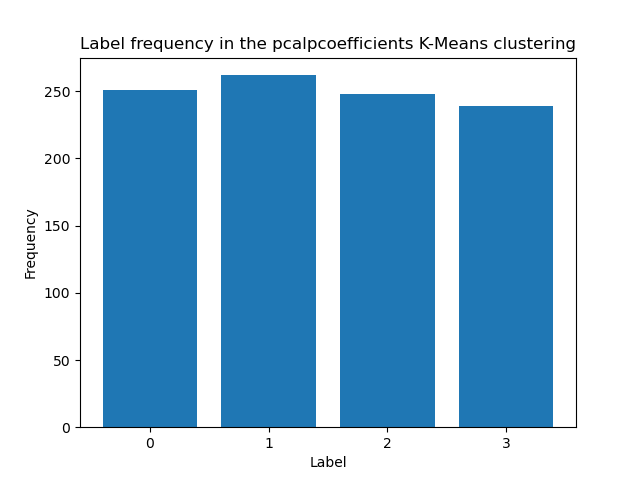
\includegraphics[width=0.45\textwidth]{mdid-pcalpcoefficientsK-Meansdensity.png}}\\
				\subfloat[Original clusters]{%
					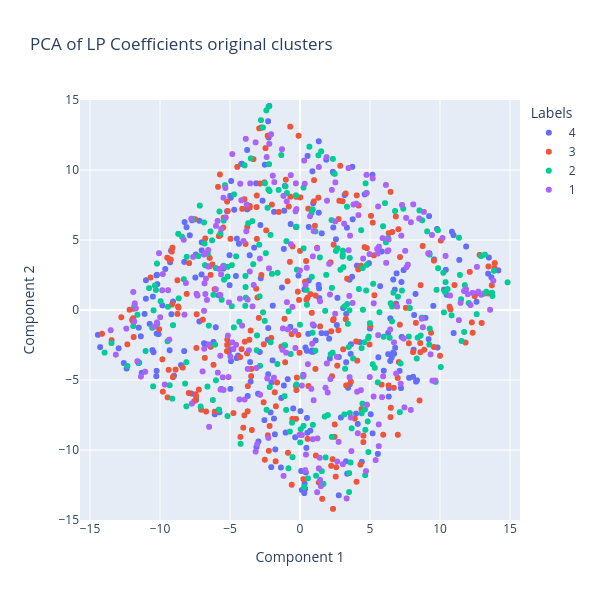
\includegraphics[width=0.45\textwidth]{mdid-pcalpcoefficientsoriginalclusters.png}}
				\hspace{\fill}
				\subfloat[K-Means clusters from PCA]{%
					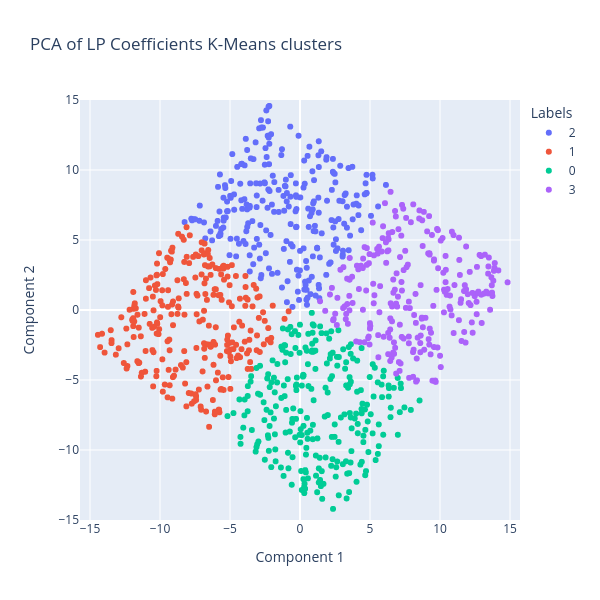
\includegraphics[width=0.45\textwidth]{mdid-pcalpcoefficientsK-Meansclusters.png}}\\
					
				\subfloat[Original cluster samples from PCA]{%
					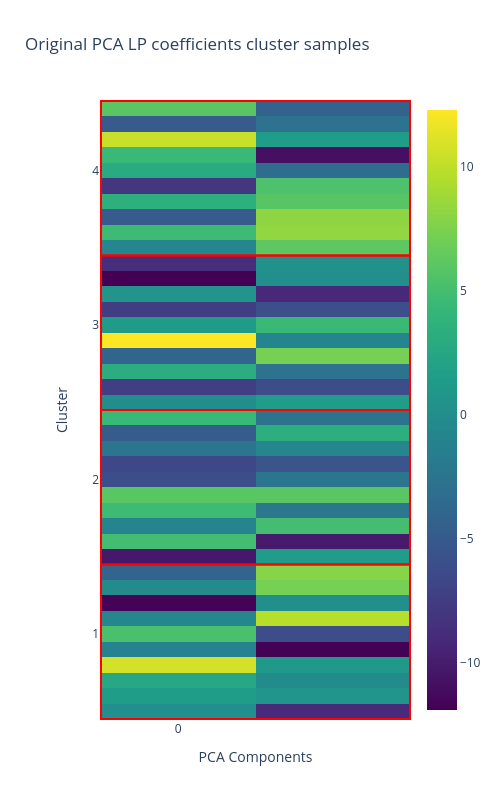
\includegraphics[width=0.4\textwidth]{mdid-pcalpcoefficientsoriginalgridclusters.png}}
				\hspace{\fill}
				\subfloat[K-Means cluster samples from PCA]{%
					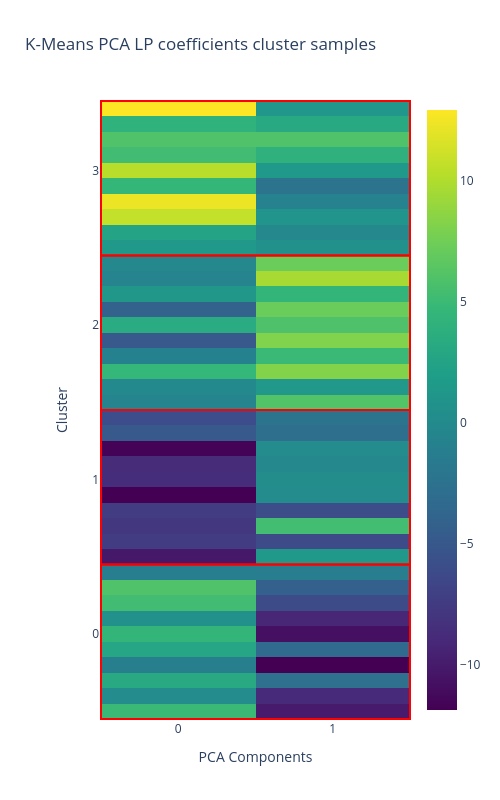
\includegraphics[width=0.4\textwidth]{mdid-pcalpcoefficientsK-Meansgridclusters.png}}
				\caption{Comparison between original clustering and K-Means clustering from PCA of LP coefficients}
			\end{figure*}
			\FloatBarrier
			
			\begin{figure*}[ht!]
				\centering
				\subfloat[Original cluster densities from UMAP]{%
					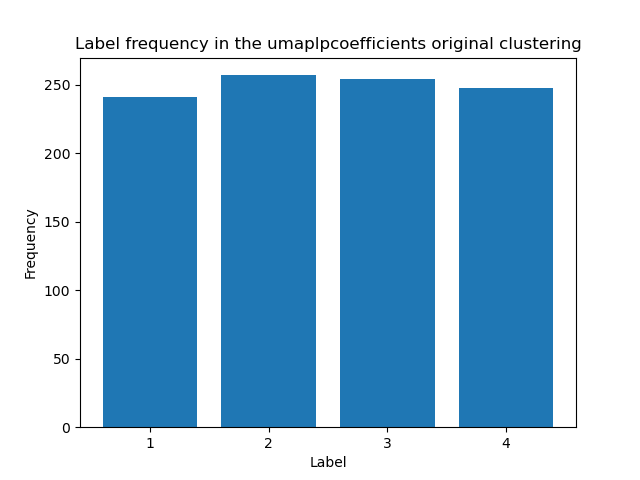
\includegraphics[width=0.45\textwidth]{mdid-umaplpcoefficientsoriginaldensity.png}}
				\hspace{\fill}
				\subfloat[K-Means clusters densities from UMAP]{%
					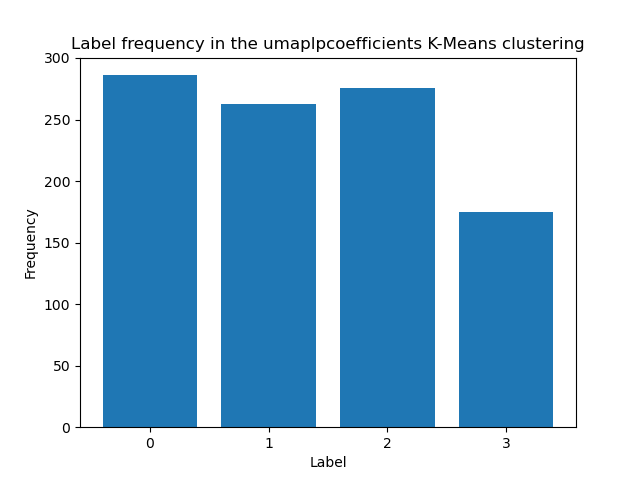
\includegraphics[width=0.45\textwidth]{mdid-umaplpcoefficientsK-Meansdensity.png}}\\
				\subfloat[Original clusters from UMAP]{%
					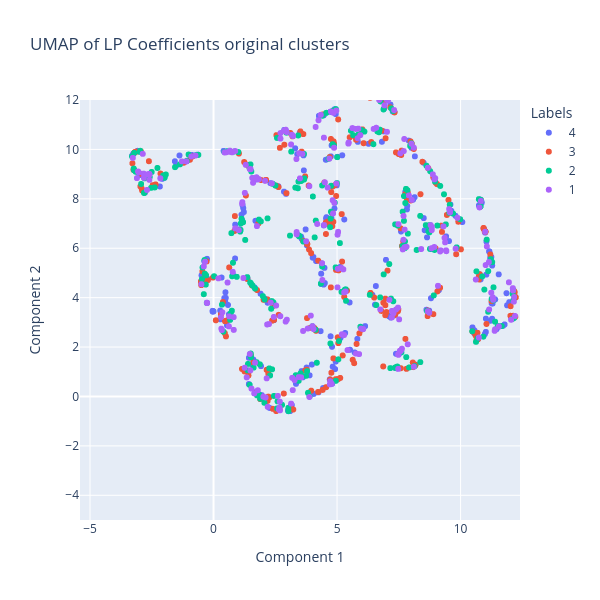
\includegraphics[width=0.45\textwidth]{mdid-umaplpcoefficientsoriginalclusters.png}}
				\hspace{\fill}
				\subfloat[K-Means clusters from UMAP]{%
					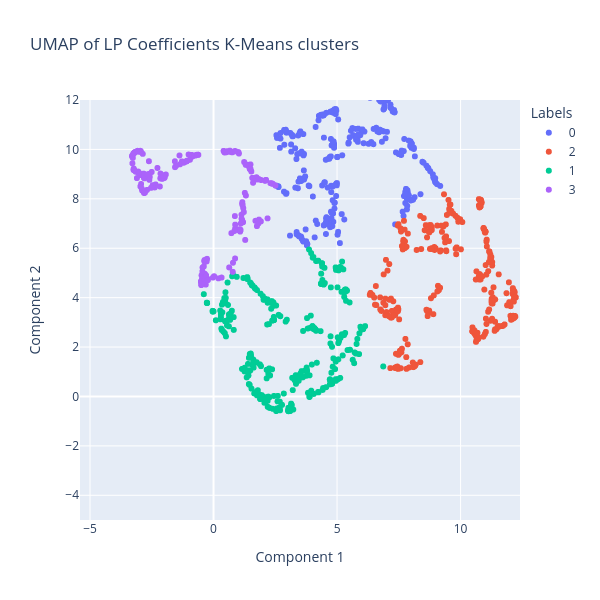
\includegraphics[width=0.45\textwidth]{mdid-umaplpcoefficientsK-Meansclusters.png}}\\
					
				\subfloat[Original cluster samples from UMAP]{%
					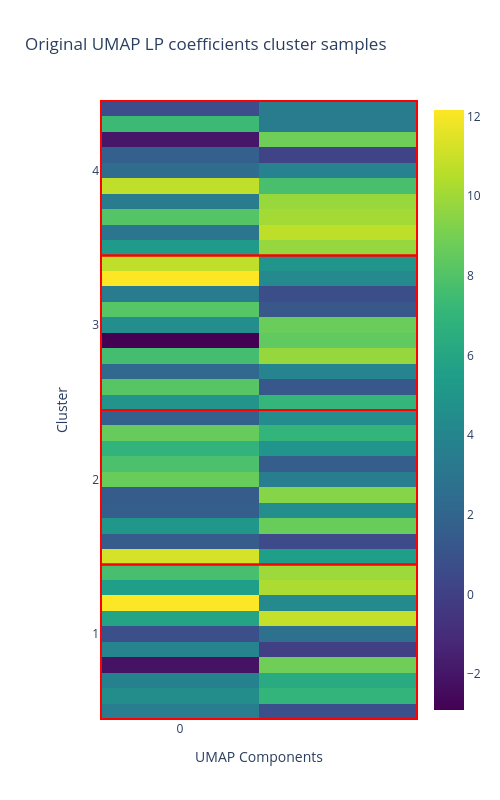
\includegraphics[width=0.4\textwidth]{mdid-umaplpcoefficientsoriginalgridclusters.png}}
				\hspace{\fill}
				\subfloat[K-Means cluster samples from UMAP]{%
					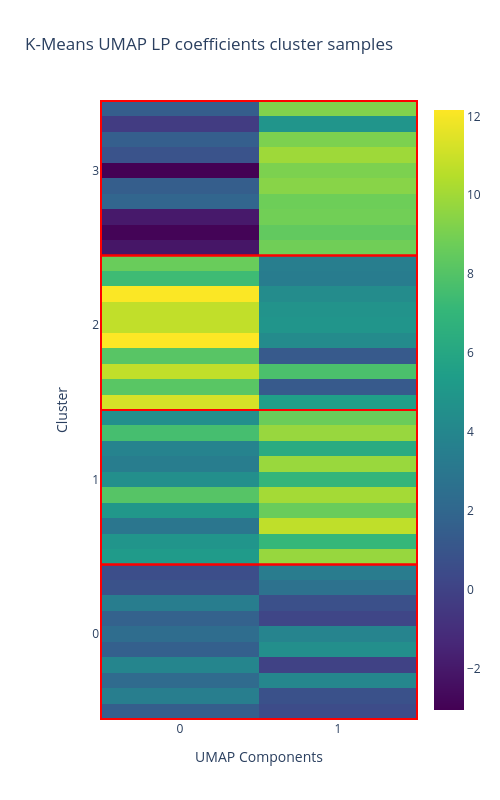
\includegraphics[width=0.4\textwidth]{mdid-umaplpcoefficientsK-Meansgridclusters.png}}
				\caption{Comparison between original clustering and K-Means clustering from UMAP of LP coefficients}
			\end{figure*}
			\FloatBarrier
		
		\subsubsection{DBSCAN}
			
			A configuration that outputs 4 clusters is searched
			
			\begin{table}[h!]
				\centering
				\begin{tabular}{|c|c|c|}
					\hline
					& \textbf{Number of neighbours} & \textbf{Epsilon}\\
					\hline
					Original LP coefficients & 15 & 1.52\\
					\hline
					PCA LP coefficients & 15 & 1.52\\
					\hline
					UMAP LP coefficients & 10 & 0.85\\
					\hline
				\end{tabular}
				\caption{DBSCAN hyperparameter configuration for LP coefficients clustering}
			\end{table}
		
			The results are the following:
			
			\begin{figure*}[ht!]
				\centering
				\subfloat[Original cluster densities]{%
					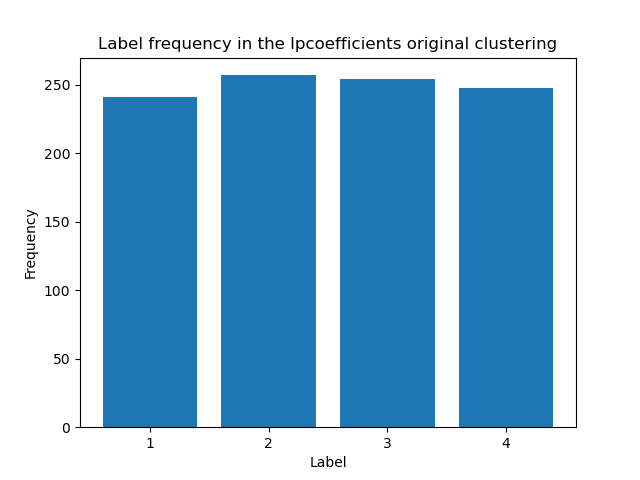
\includegraphics[width=0.45\textwidth]{mdid-lpcoefficientsoriginaldensity.png}}
				\hspace{\fill}
				\subfloat[DBSCAN clusters densities]{%
					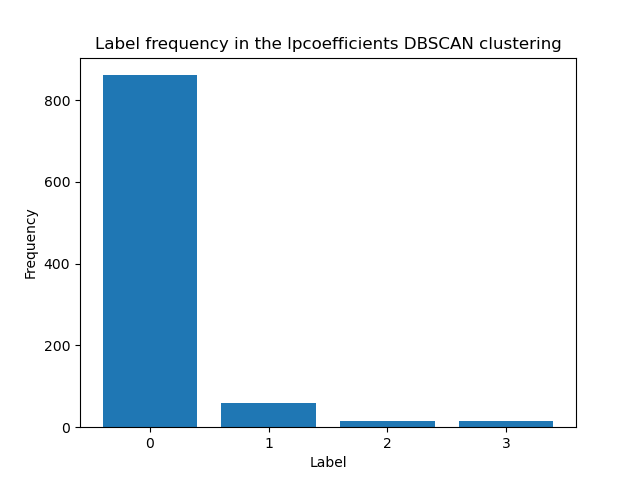
\includegraphics[width=0.45\textwidth]{mdid-lpcoefficientsDBSCANdensity.png}}
				\\
				\subfloat[Original clusters]{%
					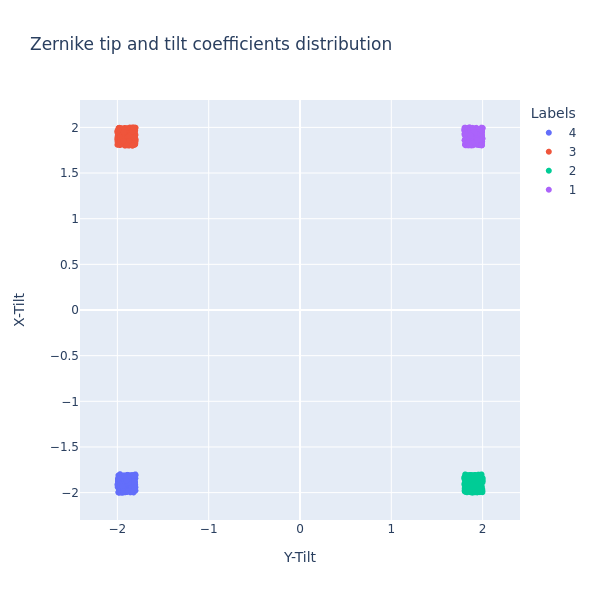
\includegraphics[width=0.45\textwidth]{mdid-originalclusters.png}}
				\hspace{\fill}
				\subfloat[DBSCAN clusters]{%
					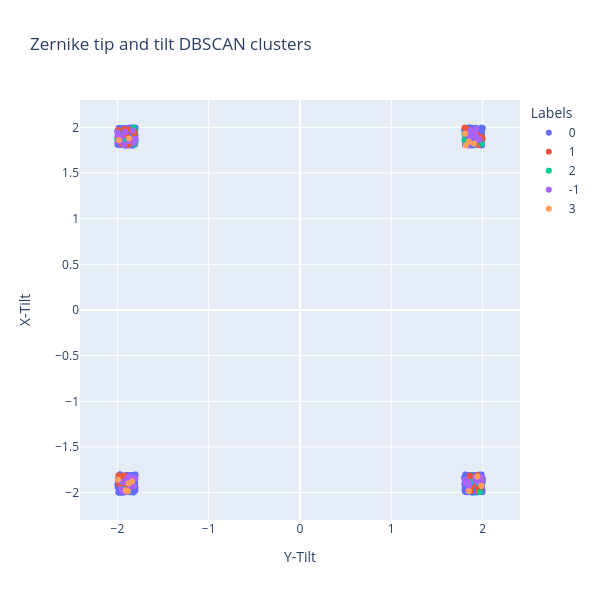
\includegraphics[width=0.45\textwidth]{mdid-lpcoefficientsDBSCANclusters.png}}\\
					
				\subfloat[Original cluster samples]{%
					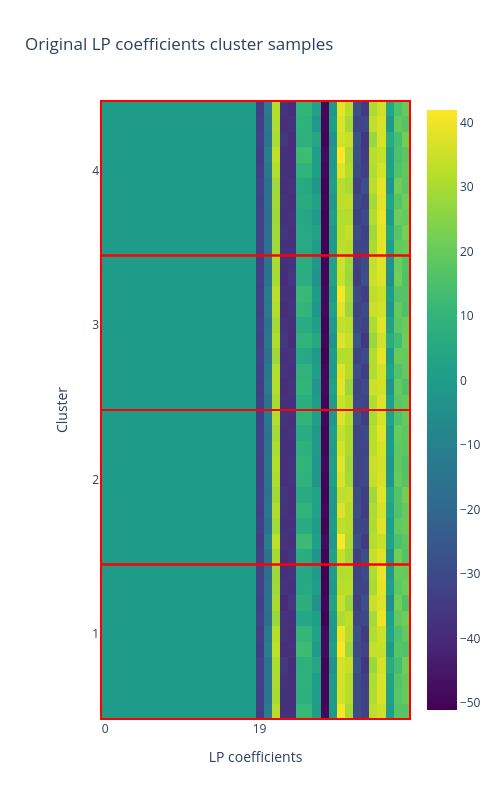
\includegraphics[width=0.4\textwidth]{mdid-lpcoefficientsoriginalgridclusters.png}}
				\hspace{\fill}
				\subfloat[DBSCAN cluster samples]{%
					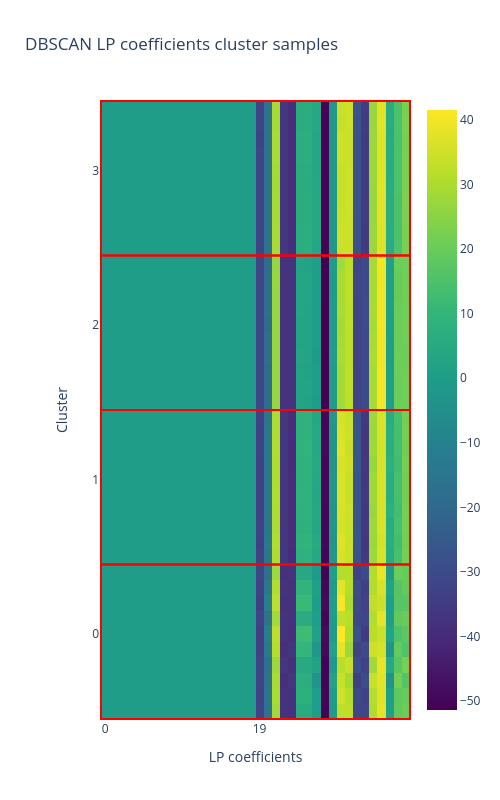
\includegraphics[width=0.4\textwidth]{mdid-lpcoefficientsDBSCANgridclusters.png}}
				\caption{Comparison between original clustering and DBSCAN clustering}
			\end{figure*}
			\FloatBarrier
			
			\begin{figure*}[ht!]
				\centering
				\subfloat[Original cluster densities from PCA]{%
					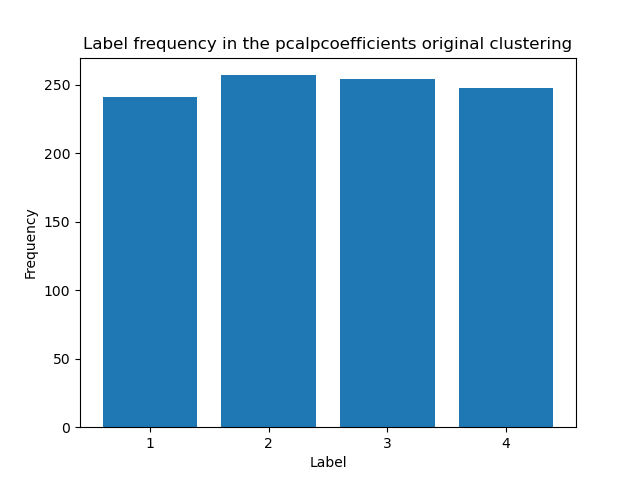
\includegraphics[width=0.45\textwidth]{mdid-pcalpcoefficientsoriginaldensity.png}}
				\hspace{\fill}
				\subfloat[DBSCAN clusters densities from PCA]{%
					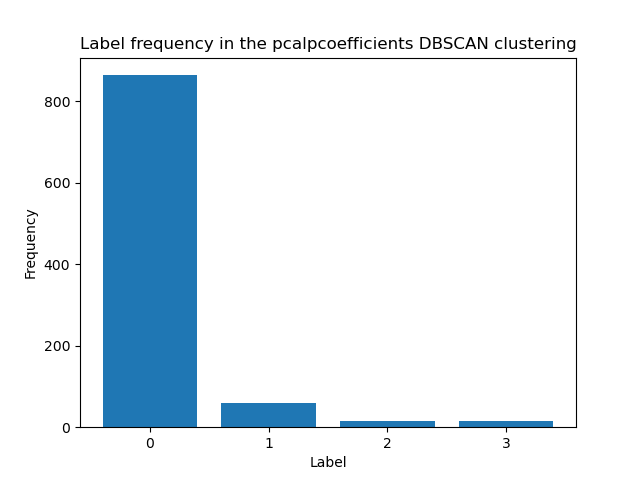
\includegraphics[width=0.45\textwidth]{mdid-pcalpcoefficientsDBSCANdensity.png}}
				\\
				\subfloat[Original clusters from PCA]{%
					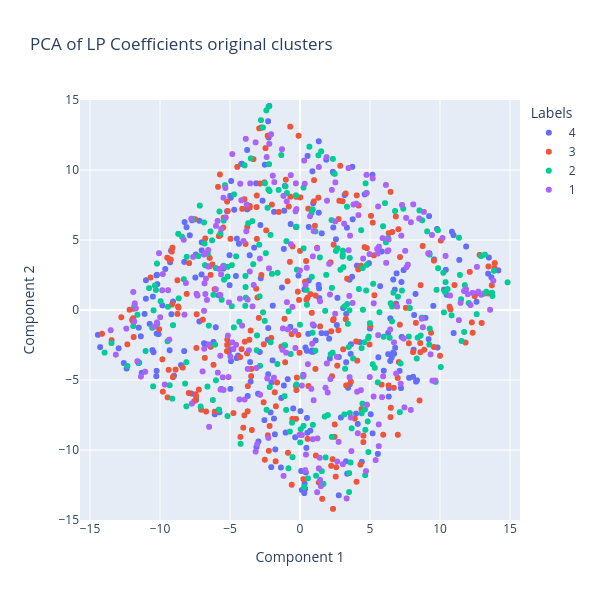
\includegraphics[width=0.45\textwidth]{mdid-pcalpcoefficientsoriginalclusters.png}}
				\hspace{\fill}
				\subfloat[DBSCAN clusters from PCA]{%
					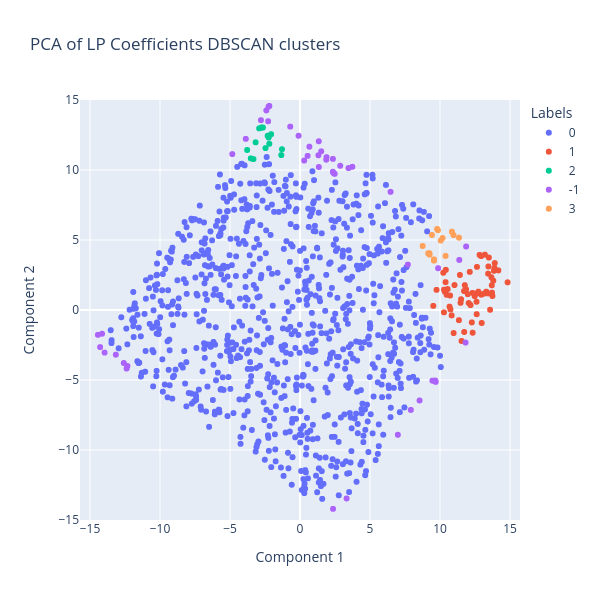
\includegraphics[width=0.45\textwidth]{mdid-pcalpcoefficientsDBSCANclusters.png}}\\
					
				\subfloat[Original cluster samples from PCA]{%
					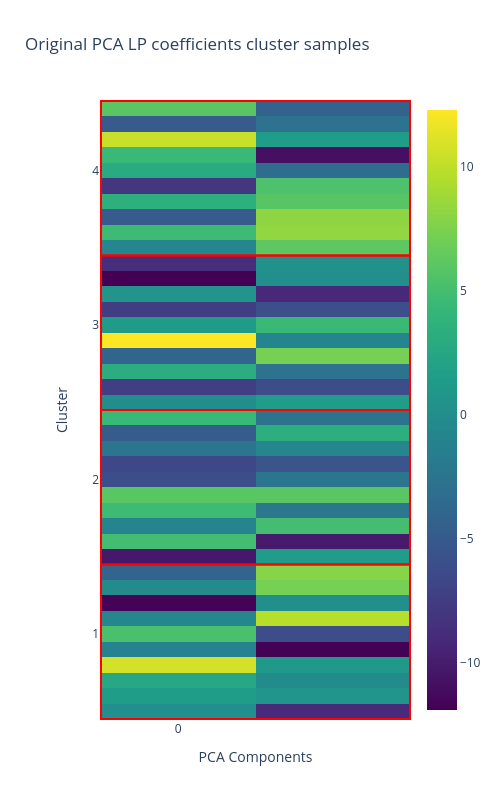
\includegraphics[width=0.4\textwidth]{mdid-pcalpcoefficientsoriginalgridclusters.png}}
				\hspace{\fill}
				\subfloat[DBSCAN cluster samples from PCA]{%
					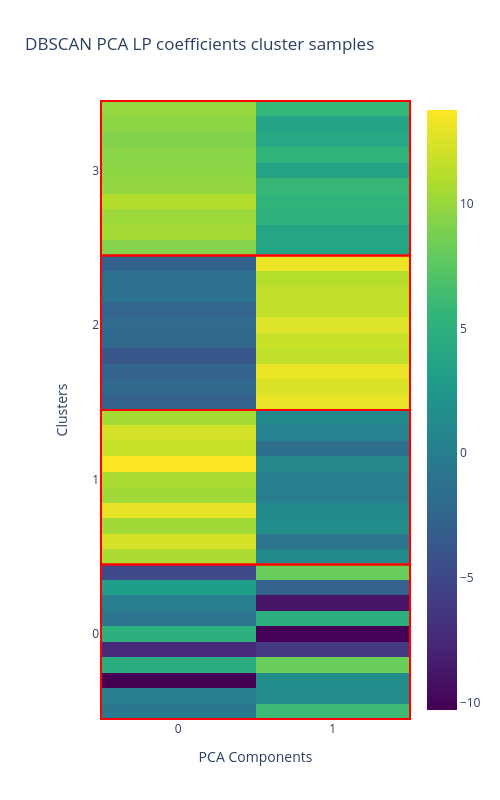
\includegraphics[width=0.4\textwidth]{mdid-pcalpcoefficientsDBSCANgridclusters.png}}
				\caption{Comparison between original clustering and DBSCAN clustering from PCA of LP coefficients}
			\end{figure*}
			\FloatBarrier
			
			\begin{figure*}[ht!]
				\centering
				\subfloat[Original cluster densities from UMAP]{%
					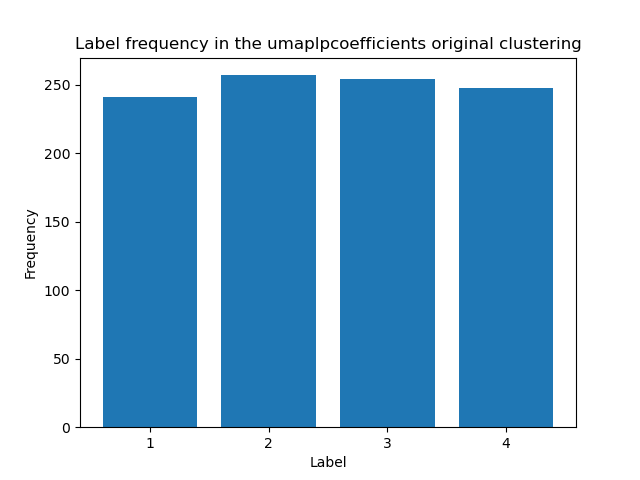
\includegraphics[width=0.45\textwidth]{mdid-umaplpcoefficientsoriginaldensity.png}}
				\hspace{\fill}
				\subfloat[DBSCAN clusters densities from UMAP]{%
					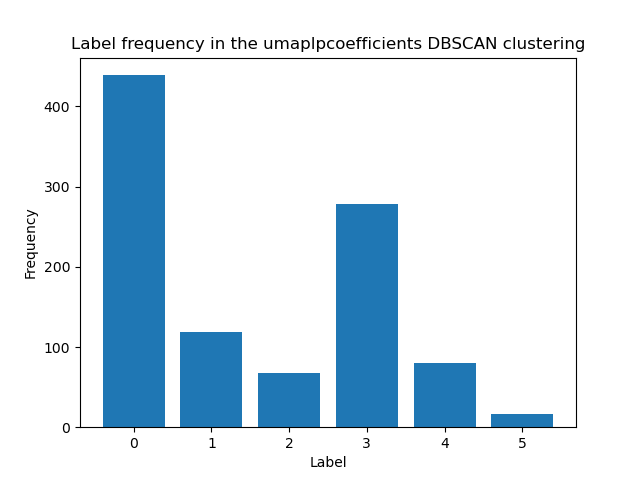
\includegraphics[width=0.45\textwidth]{mdid-umaplpcoefficientsDBSCANdensity.png}}\\
				\subfloat[Original clusters from UMAP]{%
					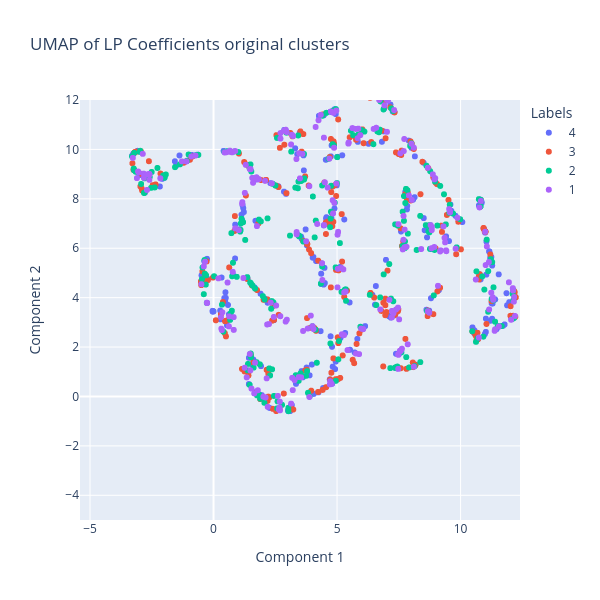
\includegraphics[width=0.45\textwidth]{mdid-umaplpcoefficientsoriginalclusters.png}}
				\hspace{\fill}
				\subfloat[DBSCAN clusters from UMAP]{%
					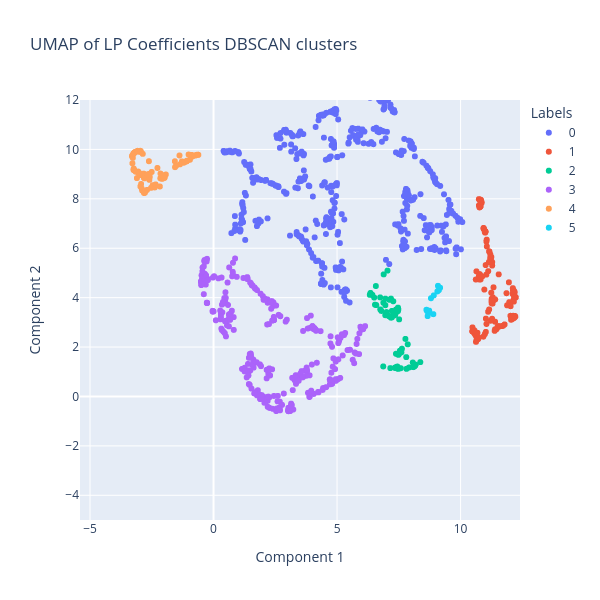
\includegraphics[width=0.45\textwidth]{mdid-umaplpcoefficientsDBSCANclusters.png}}\\
					
				\subfloat[Original cluster samples from UMAP]{%
					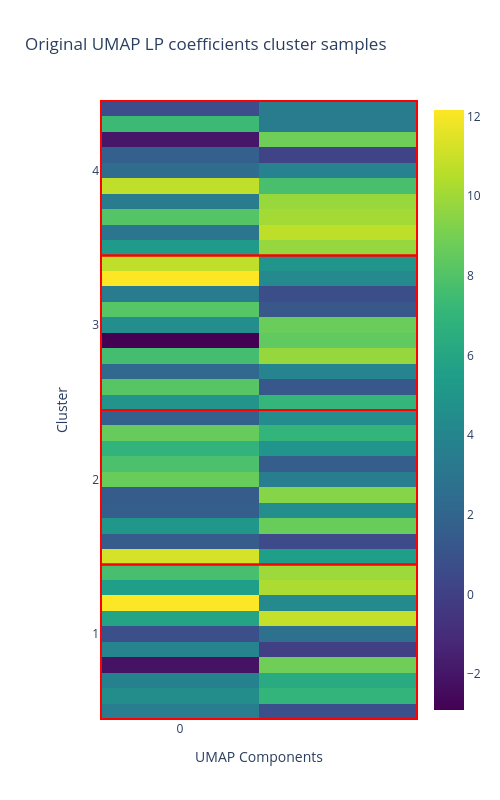
\includegraphics[width=0.4\textwidth]{mdid-umaplpcoefficientsoriginalgridclusters.png}}
				\hspace{\fill}
				\subfloat[DBSCAN cluster samples from UMAP]{%
					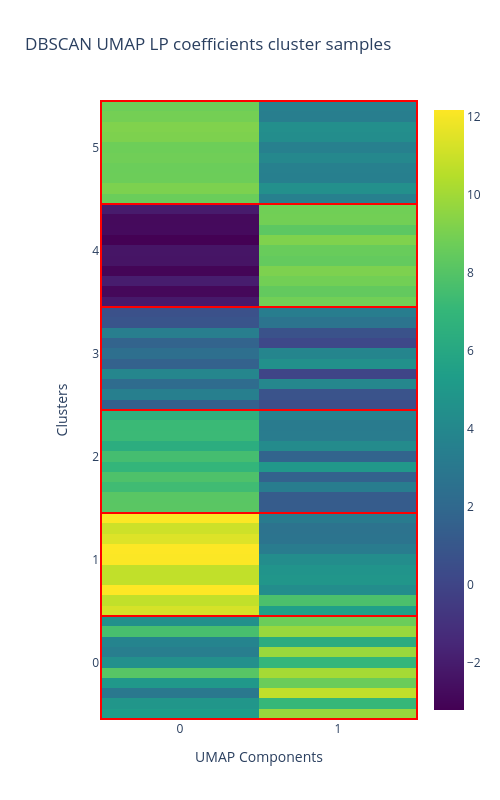
\includegraphics[width=0.4\textwidth]{mdid-umaplpcoefficientsDBSCANgridclusters.png}}
				\caption{Comparison between original clustering and DBSCAN clustering from UMAP of LP coefficients}
			\end{figure*}
			\FloatBarrier
		
		\subsubsection{HDBSCAN}
			
			A configuration that outputs 4 clusters is searched.
			
			\begin{table}[h!]
				\centering
				\begin{tabular}{|c|c|c|}
					\hline
					& \textbf{Minimum cluster size} \\
					\hline
					Original LP coefficients & 21 \\
					\hline
					PCA LP coefficients & 21 \\
					\hline
					UMAP LP coefficients & 25 \\
					\hline
				\end{tabular}
				\caption{HDBSCAN hyperparameter configuration for LP coefficients clustering}
			\end{table}
			\FloatBarrier
			
			The results are the following:
			
			\begin{figure*}[ht!]
				\centering
				\subfloat[Original cluster densities]{%
					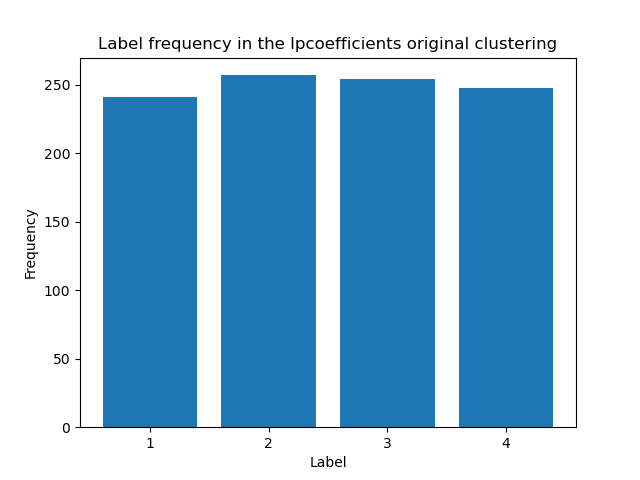
\includegraphics[width=0.45\textwidth]{mdid-lpcoefficientsoriginaldensity.png}}
				\hspace{\fill}
				\subfloat[HDBSCAN clusters densities]{%
					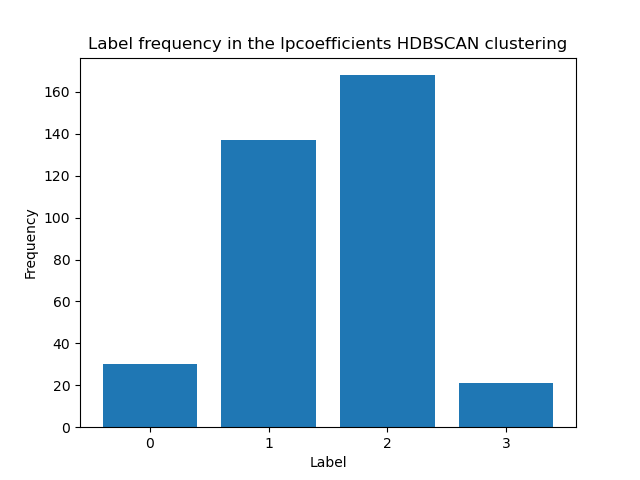
\includegraphics[width=0.45\textwidth]{mdid-lpcoefficientsHDBSCANdensity.png}}
				\\
				\subfloat[Original clusters]{%
					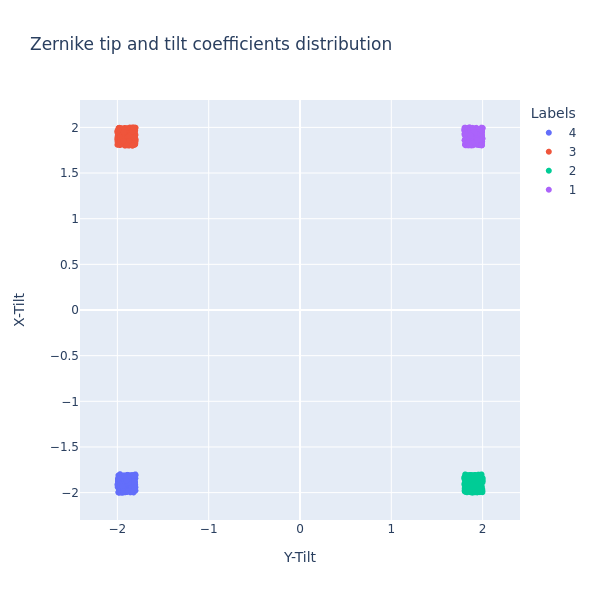
\includegraphics[width=0.45\textwidth]{mdid-originalclusters.png}}
				\hspace{\fill}
				\subfloat[HDBSCAN clusters]{%
					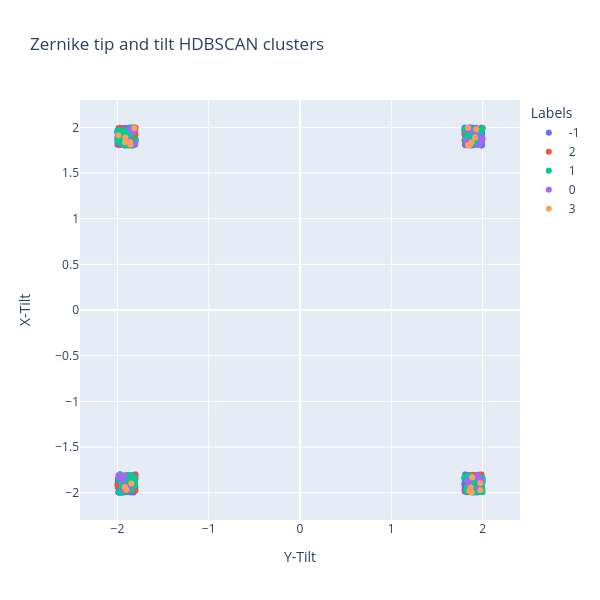
\includegraphics[width=0.45\textwidth]{mdid-lpcoefficientsHDBSCANclusters.png}}\\
					
				\subfloat[Original cluster samples]{%
					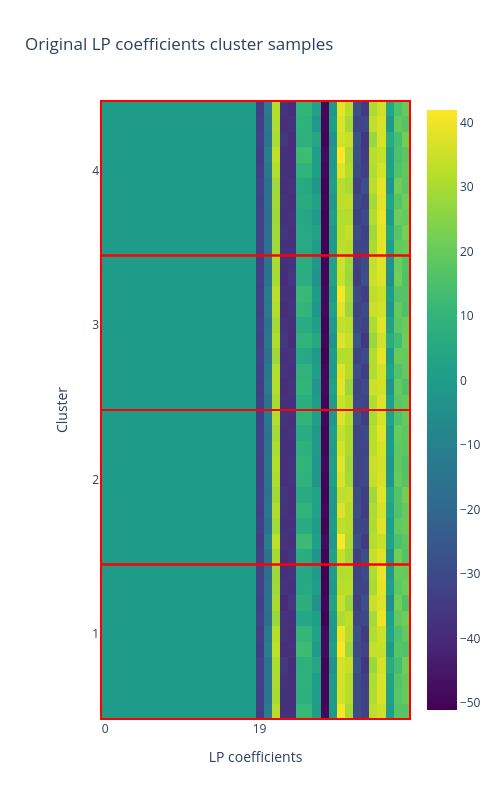
\includegraphics[width=0.4\textwidth]{mdid-lpcoefficientsoriginalgridclusters.png}}
				\hspace{\fill}
				\subfloat[HDBSCAN cluster samples]{%
					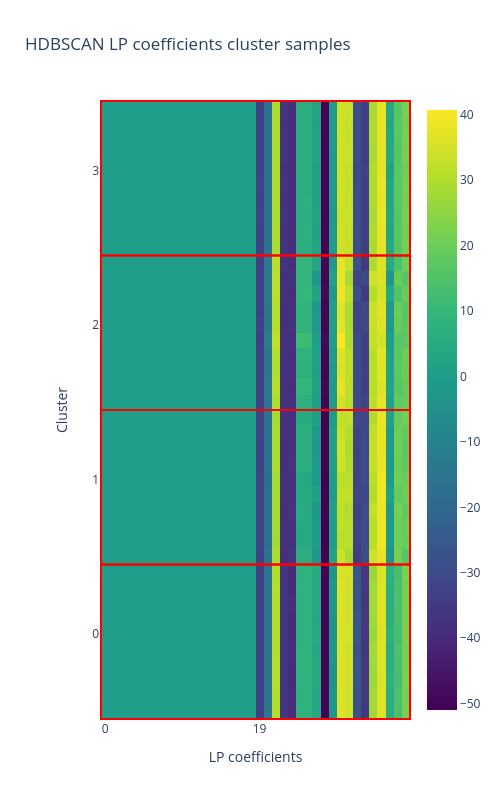
\includegraphics[width=0.4\textwidth]{mdid-lpcoefficientsHDBSCANgridclusters.png}}
				\caption{Comparison between original clustering and HDBSCAN clustering}
			\end{figure*}
			\FloatBarrier
			
			\begin{figure*}[ht!]
				\centering
				\subfloat[Original cluster densities from PCA]{%
					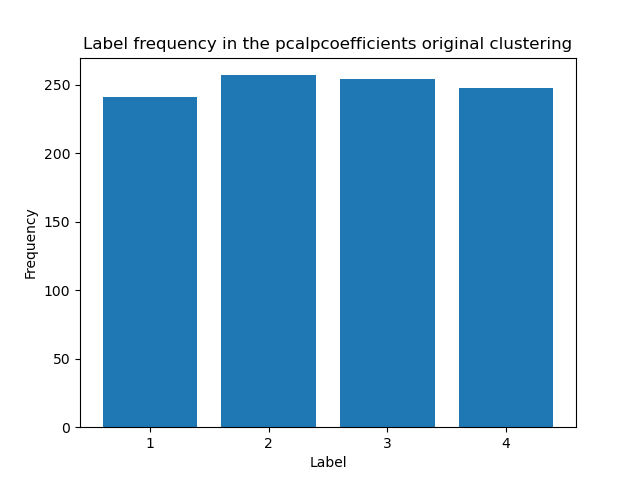
\includegraphics[width=0.45\textwidth]{mdid-pcalpcoefficientsoriginaldensity.png}}
				\hspace{\fill}
				\subfloat[HDBSCAN clusters densities from PCA]{%
					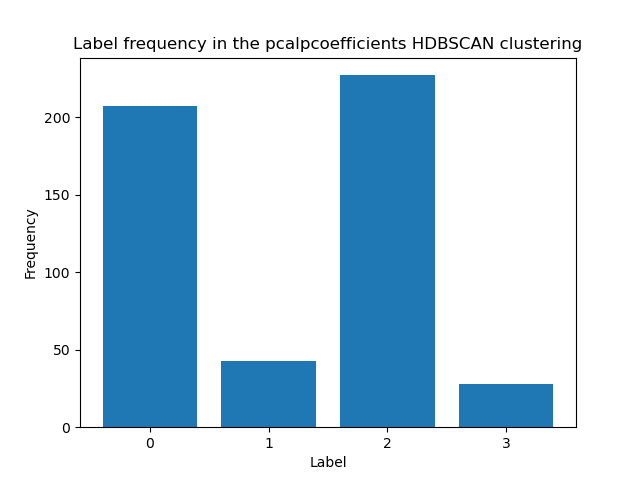
\includegraphics[width=0.45\textwidth]{mdid-pcalpcoefficientsHDBSCANdensity.png}}
				\\
				\subfloat[Original clusters from PCA]{%
					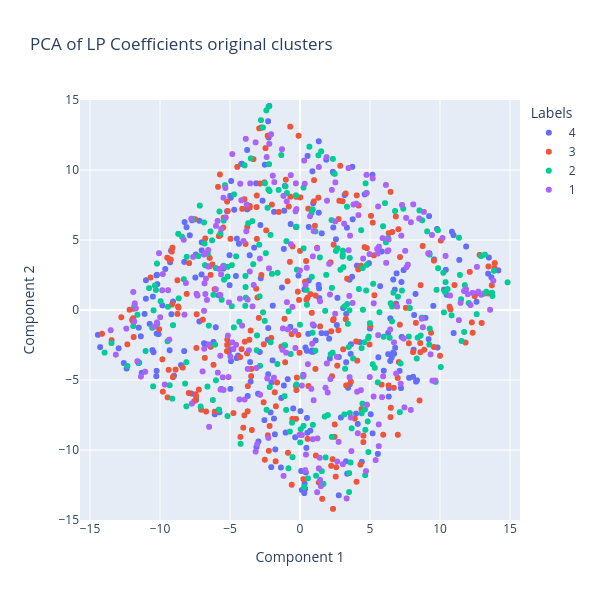
\includegraphics[width=0.45\textwidth]{mdid-pcalpcoefficientsoriginalclusters.png}}
				\hspace{\fill}
				\subfloat[HDBSCAN clusters from PCA]{%
					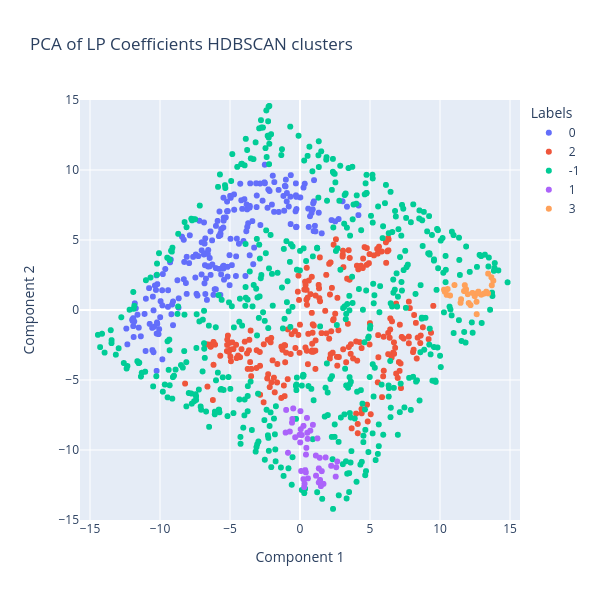
\includegraphics[width=0.45\textwidth]{mdid-pcalpcoefficientsHDBSCANclusters.png}}\\
					
				\subfloat[Original cluster samples from PCA]{%
					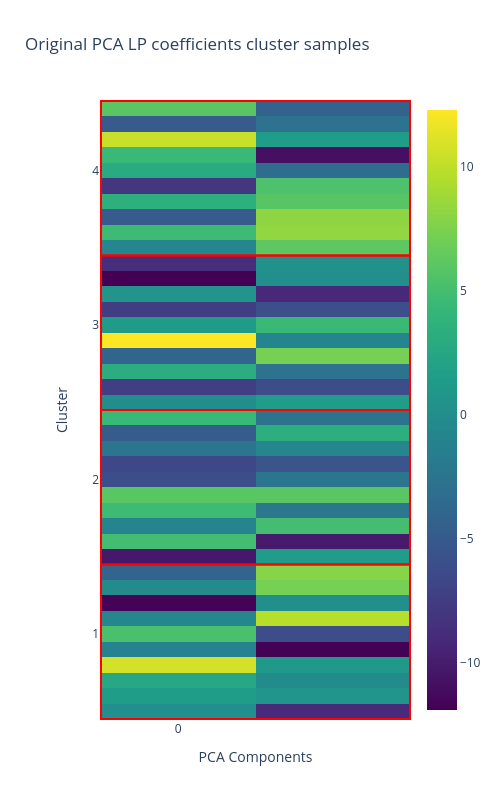
\includegraphics[width=0.4\textwidth]{mdid-pcalpcoefficientsoriginalgridclusters.png}}
				\hspace{\fill}
				\subfloat[HDBSCAN cluster samples from PCA]{%
					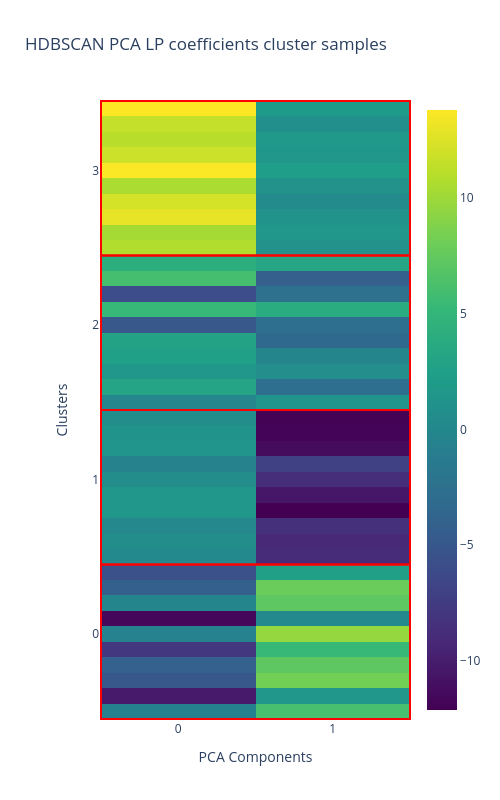
\includegraphics[width=0.4\textwidth]{mdid-pcalpcoefficientsHDBSCANgridclusters.png}}
				\caption{Comparison between original clustering and HDBSCAN clustering from PCA of LP coefficients}
			\end{figure*}
			\FloatBarrier
			
			\begin{figure*}[ht!]
				\centering
				\subfloat[Original cluster densities from UMAP]{%
					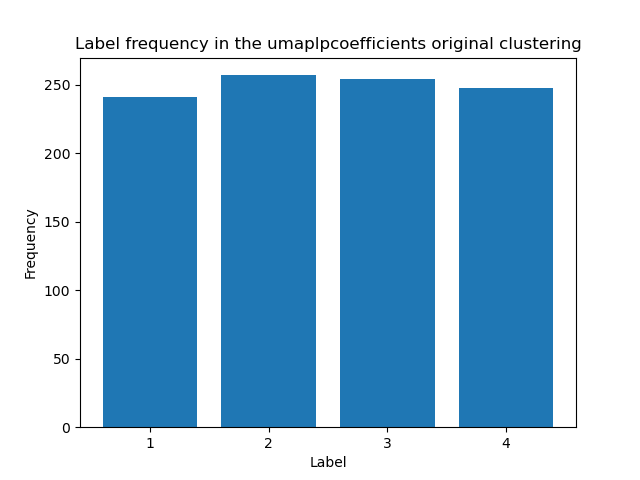
\includegraphics[width=0.45\textwidth]{mdid-umaplpcoefficientsoriginaldensity.png}}
				\hspace{\fill}
				\subfloat[HDBSCAN clusters densities from UMAP]{%
					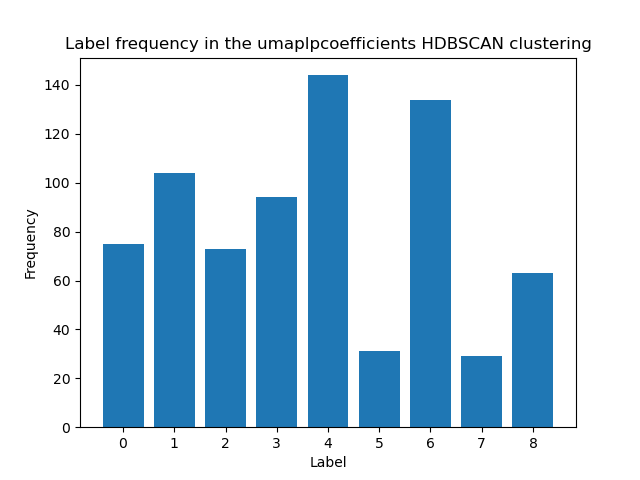
\includegraphics[width=0.45\textwidth]{mdid-umaplpcoefficientsHDBSCANdensity.png}}\\
				\subfloat[Original clusters from UMAP]{%
					\includegraphics[width=0.45\textwidth]{mdid-umaplpcoefficientsoriginalclusters.png}}
				\hspace{\fill}
				\subfloat[HDBSCAN clusters from UMAP]{%
					\includegraphics[width=0.45\textwidth]{mdid-umaplpcoefficientsHDBSCANclusters.png}}\\
					
				\subfloat[Original cluster samples from UMAP]{%
					\includegraphics[width=0.4\textwidth]{mdid-umaplpcoefficientsoriginalgridclusters.png}}
				\hspace{\fill}
				\subfloat[HDBSCAN cluster samples from UMAP]{%
					\includegraphics[width=0.4\textwidth]{mdid-umaplpcoefficientsHDBSCANgridclusters.png}}
				\caption{Comparison between original clustering and HDBSCAN clustering from UMAP of LP coefficients}
			\end{figure*}
			\FloatBarrier
		
		\subsubsection{Agglomerative clustering}
			\begin{table}[h!]
				\centering
				\begin{tabular}{|c|c|}
					\hline
					 & \textbf{Number of clusters} \\
					\hline
					Original LP coefficients & 4 \\
					\hline
					PCA LP coefficients & 4 \\
					\hline
					UMAP LP coefficients & 4 \\
					\hline
				\end{tabular}
				\caption{Agglomerative hyperparameter configuration for LP coefficients clustering}
			\end{table}
			\FloatBarrier
			The results are the following:
			
			\begin{figure*}[ht!]
				\centering
				\subfloat[Original cluster densities]{%
					\includegraphics[width=0.45\textwidth]{mdid-lpcoefficientsoriginaldensity.png}}
				\hspace{\fill}
				\subfloat[Agglomerative clusters densities]{%
					\includegraphics[width=0.45\textwidth]{mdid-lpcoefficientsAgglomerativedensity.png}}
				\\
				\subfloat[Original clusters]{%
					\includegraphics[width=0.45\textwidth]{mdid-originalclusters.png}}
				\hspace{\fill}
				\subfloat[Agglomerative clusters]{%
					\includegraphics[width=0.45\textwidth]{mdid-lpcoefficientsAgglomerativeclusters.png}}\\
					
				\subfloat[Original cluster samples]{%
					\includegraphics[width=0.4\textwidth]{mdid-lpcoefficientsoriginalgridclusters.png}}
				\hspace{\fill}
				\subfloat[Agglomerative cluster samples]{%
					\includegraphics[width=0.4\textwidth]{mdid-lpcoefficientsAgglomerativegridclusters.png}}
				\caption{Comparison between original clustering and Agglomerative clustering}
			\end{figure*}
			\FloatBarrier
			
			\begin{figure*}[ht!]
				\centering
				\subfloat[Original cluster densities from PCA]{%
					\includegraphics[width=0.45\textwidth]{mdid-pcalpcoefficientsoriginaldensity.png}}
				\hspace{\fill}
				\subfloat[Agglomerative clusters densities from PCA]{%
					\includegraphics[width=0.45\textwidth]{mdid-pcalpcoefficientsAgglomerativedensity.png}}
				\\
				\subfloat[Original clusters from PCA]{%
					\includegraphics[width=0.45\textwidth]{mdid-pcalpcoefficientsoriginalclusters.png}}
				\hspace{\fill}
				\subfloat[Agglomerative clusters from PCA]{%
					\includegraphics[width=0.45\textwidth]{mdid-pcalpcoefficientsAgglomerativeclusters.png}}\\
					
				\subfloat[Original cluster samples from PCA]{%
					\includegraphics[width=0.4\textwidth]{mdid-pcalpcoefficientsoriginalgridclusters.png}}
				\hspace{\fill}
				\subfloat[Agglomerative cluster samples from PCA]{%
					\includegraphics[width=0.4\textwidth]{mdid-pcalpcoefficientsAgglomerativegridclusters.png}}
				\caption{Comparison between original clustering and Agglomerative clustering}
			\end{figure*}
			\FloatBarrier
			
			\begin{figure*}[ht!]
				\centering
				\subfloat[Original cluster densities from UMAP]{%
					\includegraphics[width=0.45\textwidth]{mdid-umaplpcoefficientsoriginaldensity.png}}
				\hspace{\fill}
				\subfloat[Agglomerative clusters densities from UMAP]{%
					\includegraphics[width=0.45\textwidth]{mdid-umaplpcoefficientsAgglomerativedensity.png}}\\
				\subfloat[Original clusters from UMAP]{%
					\includegraphics[width=0.45\textwidth]{mdid-umaplpcoefficientsoriginalclusters.png}}
				\hspace{\fill}
				\subfloat[Agglomerative clusters from UMAP]{%
					\includegraphics[width=0.45\textwidth]{mdid-umaplpcoefficientsAgglomerativeclusters.png}}\\
					
				\subfloat[Original cluster samples from UMAP]{%
					\includegraphics[width=0.4\textwidth]{mdid-umaplpcoefficientsoriginalgridclusters.png}}
				\hspace{\fill}
				\subfloat[Agglomerative cluster samples from UMAP]{%
					\includegraphics[width=0.4\textwidth]{mdid-umaplpcoefficientsAgglomerativegridclusters.png}}
				\caption{Comparison between original clustering and Agglomerative clustering from UMAP of LP coefficients}
			\end{figure*}
			\FloatBarrier
		
		\subsubsection{Summary}
			\begin{figure*}[ht!]
				\centering
				\subfloat[Original cluster densities]{%
					\includegraphics[width=0.18\textwidth]{mdid-lpcoefficientsoriginaldensity.png}}
				\hspace{\fill}
				\subfloat[K-means cluster densities]{%
					\includegraphics[width=0.18\textwidth]{mdid-lpcoefficientsK-Meansdensity.png}}
				\hspace{\fill}
				\subfloat[DBSCAN cluster densities]{%
					\includegraphics[width=0.18\textwidth]{mdid-lpcoefficientsDBSCANdensity.png}}
				\hspace{\fill}
				\subfloat[HDBSCAN cluster densities]{%
					\includegraphics[width=0.18\textwidth]{mdid-lpcoefficientsHDBSCANdensity.png}}
				\hspace{\fill}
				\subfloat[Agglomerative cluster densities]{%
					\includegraphics[width=0.18\textwidth]{mdid-lpcoefficientsAgglomerativedensity.png}}
				\\
				
				\subfloat[Original cluster]{%
					\includegraphics[width=0.18\textwidth]{mdid-originalclusters.png}}
				\hspace{\fill}
				\subfloat[K-means clusters]{%
					\includegraphics[width=0.18\textwidth]{mdid-lpcoefficientsK-Meansclusters.png}}
				\hspace{\fill}
				\subfloat[DBSCAN cluster clusters]{%
					\includegraphics[width=0.18\textwidth]{mdid-lpcoefficientsDBSCANclusters.png}}
				\hspace{\fill}
				\subfloat[HDBSCAN clusters]{%
					\includegraphics[width=0.18\textwidth]{mdid-lpcoefficientsHDBSCANclusters.png}}
				\hspace{\fill}
				\subfloat[Agglomerative clusters]{%
					\includegraphics[width=0.18\textwidth]{mdid-lpcoefficientsAgglomerativeclusters.png}}\\
				
				\subfloat[Original cluster samples]{%
					\includegraphics[width=0.18\textwidth]{mdid-lpcoefficientsoriginalgridclusters.png}}
				\hspace{\fill}
				\subfloat[K-means cluster samples]{%
					\includegraphics[width=0.18\textwidth]{mdid-lpcoefficientsK-Meansgridclusters.png}}
				\hspace{\fill}
				\subfloat[DBSCAN cluster samples]{%
					\includegraphics[width=0.18\textwidth]{mdid-lpcoefficientsDBSCANgridclusters.png}}
				\hspace{\fill}
				\subfloat[HDBSCAN cluster samples]{%
					\includegraphics[width=0.18\textwidth]{mdid-lpcoefficientsHDBSCANgridclusters.png}}
				\hspace{\fill}
				\subfloat[Agglomerative cluster samples]{%
					\includegraphics[width=0.18\textwidth]{mdid-lpcoefficientsAgglomerativegridclusters.png}}
				
				\caption{Comparison between clustering LP coefficients algorithms}
			\end{figure*}
		\FloatBarrier
		
		\begin{table}[h!]
    			\centering
    			\begin{tabular}{|c|c|c|c|c|c|}
        			\hline
        			& \textbf{Original} & \textbf{K-Means} & \textbf{DBSCAN} & \textbf{HDBSCAN} & \textbf{Agglomerative} \\
        			\hline
        			\textbf{Original} & \diagbox{}{} & 0.002 & 0.008 & 0.004 & 0.002 \\
       			\hline
        			\textbf{K-Means} &  & \diagbox{}{} & 0.154 & 0.143 & 0.695\\
        			\hline
        			\textbf{DBSCAN} &  &  & \diagbox{}{} & 0.175 & 0.142\\
        			\hline
        			\textbf{HDBSCAN} &  &  &  & \diagbox{}{} & 0.002\\
       			\hline
    			\end{tabular}
    			\caption{Normalized Mutual Information between original LP coefficients clusters}
		\end{table}
		
		\begin{figure*}[ht!]
				\centering
				\subfloat[Original cluster densities from PCA]{%
					\includegraphics[width=0.18\textwidth]{mdid-pcalpcoefficientsoriginaldensity.png}}
				\hspace{\fill}
				\subfloat[K-means cluster densities from PCA]{%
					\includegraphics[width=0.18\textwidth]{mdid-pcalpcoefficientsK-Meansdensity.png}}
				\hspace{\fill}
				\subfloat[DBSCAN cluster densities from PCA]{%
					\includegraphics[width=0.18\textwidth]{mdid-pcalpcoefficientsDBSCANdensity.png}}
				\hspace{\fill}
				\subfloat[HDBSCAN cluster densities from PCA]{%
					\includegraphics[width=0.18\textwidth]{mdid-pcalpcoefficientsHDBSCANdensity.png}}
				\hspace{\fill}
				\subfloat[Agglomerative cluster densities from PCA]{%
					\includegraphics[width=0.18\textwidth]{mdid-pcalpcoefficientsAgglomerativedensity.png}}
				\\
				
				\subfloat[Original cluster from PCA]{%
					\includegraphics[width=0.18\textwidth]{mdid-pcalpcoefficientsoriginalclusters.png}}
				\hspace{\fill}
				\subfloat[K-means clusters from PCA]{%
					\includegraphics[width=0.18\textwidth]{mdid-pcalpcoefficientsK-Meansclusters.png}}
				\hspace{\fill}
				\subfloat[DBSCAN cluster clusters from PCA]{%
					\includegraphics[width=0.18\textwidth]{mdid-pcalpcoefficientsDBSCANclusters.png}}
				\hspace{\fill}
				\subfloat[HDBSCAN clusters from PCA]{%
					\includegraphics[width=0.18\textwidth]{mdid-pcalpcoefficientsHDBSCANclusters.png}}
				\hspace{\fill}
				\subfloat[Agglomerative clusters from PCA]{%
					\includegraphics[width=0.18\textwidth]{mdid-pcalpcoefficientsAgglomerativeclusters.png}}\\
				
				\subfloat[Original cluster samples from PCA]{%
					\includegraphics[width=0.18\textwidth]{mdid-pcalpcoefficientsoriginalgridclusters.png}}
				\hspace{\fill}
				\subfloat[K-means cluster samples from PCA]{%
					\includegraphics[width=0.18\textwidth]{mdid-pcalpcoefficientsK-Meansgridclusters.png}}
				\hspace{\fill}
				\subfloat[DBSCAN cluster samplesfrom PCA]{%
					\includegraphics[width=0.18\textwidth]{mdid-pcalpcoefficientsDBSCANgridclusters.png}}
				\hspace{\fill}
				\subfloat[HDBSCAN cluster samples from PCA]{%
					\includegraphics[width=0.18\textwidth]{mdid-pcalpcoefficientsHDBSCANgridclusters.png}}
				\hspace{\fill}
				\subfloat[Agglomerative cluster samples from PCA]{%
					\includegraphics[width=0.18\textwidth]{mdid-pcalpcoefficientsAgglomerativegridclusters.png}}
				
				\caption{Comparison between clustering PCA LP coefficients algorithms}
			\end{figure*}
		\FloatBarrier
		
		\begin{table}[h!]
    			\centering
    			\begin{tabular}{|c|c|c|c|c|c|}
        			\hline
        			& \textbf{Original} & \textbf{K-Means} & \textbf{DBSCAN} & \textbf{HDBSCAN} & \textbf{Agglomerative} \\
        			\hline
        			\textbf{Original} & \diagbox{}{} & 0.002 & 0.003 & 0.004 & 0.003 \\
       			\hline
        			\textbf{K-Means} &  & \diagbox{}{} & 0.150 & 0.143 & 0.642\\
        			\hline
        			\textbf{DBSCAN} &  &  & \diagbox{}{} & 0.174 & 0.209\\
        			\hline
        			\textbf{HDBSCAN} &  &  &  & \diagbox{}{} & 0.003\\
       			\hline
    			\end{tabular}
    			\caption{Normalized Mutual Information between PCA LP coefficients clusters}
		\end{table}
		
		\begin{figure*}[ht!]
				\centering
				\subfloat[Original cluster densities from UMAP]{%
					\includegraphics[width=0.18\textwidth]{mdid-umaplpcoefficientsoriginaldensity.png}}
				\hspace{\fill}
				\subfloat[K-means cluster densities from UMAP]{%
					\includegraphics[width=0.18\textwidth]{mdid-umaplpcoefficientsK-Meansdensity.png}}
				\hspace{\fill}
				\subfloat[DBSCAN cluster densities from UMAP]{%
					\includegraphics[width=0.18\textwidth]{mdid-umaplpcoefficientsDBSCANdensity.png}}
				\hspace{\fill}
				\subfloat[HDBSCAN cluster densities from UMAP]{%
					\includegraphics[width=0.18\textwidth]{mdid-umaplpcoefficientsHDBSCANdensity.png}}
				\hspace{\fill}
				\subfloat[Agglomerative cluster densities from UMAP]{%
					\includegraphics[width=0.18\textwidth]{mdid-umaplpcoefficientsAgglomerativedensity.png}}
				\\
				
				\subfloat[Original cluster from UMAP]{%
					\includegraphics[width=0.18\textwidth]{mdid-umaplpcoefficientsoriginalclusters.png}}
				\hspace{\fill}
				\subfloat[K-means clusters from UMAP]{%
					\includegraphics[width=0.18\textwidth]{mdid-umaplpcoefficientsK-Meansclusters.png}}
				\hspace{\fill}
				\subfloat[DBSCAN cluster clusters from UMAP]{%
					\includegraphics[width=0.18\textwidth]{mdid-umaplpcoefficientsDBSCANclusters.png}}
				\hspace{\fill}
				\subfloat[HDBSCAN clusters from UMAP]{%
					\includegraphics[width=0.18\textwidth]{mdid-umaplpcoefficientsHDBSCANclusters.png}}
				\hspace{\fill}
				\subfloat[Agglomerative clusters from UMAP]{%
					\includegraphics[width=0.18\textwidth]{mdid-umaplpcoefficientsAgglomerativeclusters.png}}\\
				
				\subfloat[Original cluster samples from UMAP]{%
					\includegraphics[width=0.18\textwidth]{mdid-umaplpcoefficientsoriginalgridclusters.png}}
				\hspace{\fill}
				\subfloat[K-means cluster samples from UMAP]{%
					\includegraphics[width=0.18\textwidth]{mdid-umaplpcoefficientsK-Meansgridclusters.png}}
				\hspace{\fill}
				\subfloat[DBSCAN cluster samplesfrom UMAP]{%
					\includegraphics[width=0.18\textwidth]{mdid-umaplpcoefficientsDBSCANgridclusters.png}}
				\hspace{\fill}
				\subfloat[HDBSCAN cluster samples from UMAP]{%
					\includegraphics[width=0.18\textwidth]{mdid-umaplpcoefficientsHDBSCANgridclusters.png}}
				\hspace{\fill}
				\subfloat[Agglomerative cluster samples from UMAP]{%
					\includegraphics[width=0.18\textwidth]{mdid-umaplpcoefficientsAgglomerativegridclusters.png}}
				
				\caption{Comparison between clustering UMAP LP coefficients algorithms}
			\end{figure*}
		\FloatBarrier
		
		\begin{table}[h!]
    			\centering
    			\begin{tabular}{|c|c|c|c|c|c|}
        			\hline
        			& \textbf{Original} & \textbf{K-Means} & \textbf{DBSCAN} & \textbf{HDBSCAN} & \textbf{Agglomerative} \\
        			\hline
        			\textbf{Original} & \diagbox{}{} & 0.003 & 0.001 & 0.009 & 0.001 \\
       			\hline
        			\textbf{K-Means} &  & \diagbox{}{} & 0.438 & 0.480 & 0.667\\
        			\hline
        			\textbf{DBSCAN} &  &  & \diagbox{}{} & 0.487 & 0.529\\
        			\hline
        			\textbf{HDBSCAN} &  &  &  & \diagbox{}{} & 0.001\\
       			\hline
    			\end{tabular}
    			\caption{Normalized Mutual Information between UMAP LP coefficients clusters}
		\end{table}